This chapter details the implementation of each UrbanPulse microservice, tracing
the data path from raw API polling through streaming ingestion, lakehouse
persistence, machine learning inference, and finally the serving layer that
delivers results to the frontend.

% ============================================================
\section{Ingestion Service}
\label{sec:impl-ingestion}
% ============================================================

The \textbf{Ingestion Service} is a long-running Python process that polls the
\textbf{VietMap Directions API} every \textbf{5 minutes} for 20 predefined
inter-zone routes across Ho Chi Minh City. Each route is defined by an origin
and destination anchor point (WGS-84 latitude/longitude pair) together with
a human-readable zone label.

\subsection{VietMap API Integration}

The \texttt{sources/vietmap.py} module constructs a REST request to the
\texttt{/api/route/v3} endpoint, requesting \texttt{congestion} annotations
per road segment:

\begin{lstlisting}[language=Python,
  caption={VietMap congestion metric extraction.},
  label={lst:vietmap}]
def _calc_congestion(segments: list[dict]) -> CongestionMetrics:
    total = len(segments)
    counts = {"heavy": 0, "moderate": 0, "low": 0, "severe": 0}
    for seg in segments:
        v = seg.get("value", "")
        if v in counts:
            counts[v] += 1
    return CongestionMetrics(
        heavy_ratio=round(counts["heavy"] / total, 3),
        moderate_ratio=round(counts["moderate"] / total, 3),
        severe_segments=counts["severe"],
        total_segments=total,
    )
\end{lstlisting}

\noindent The resulting \texttt{TrafficRouteObservation} object is serialised to
JSON and published to the Redpanda topic \texttt{traffic-route-bronze} with a
Kafka header \texttt{ingest\_ts} (Unix milliseconds) attached for downstream
lag measurement.

Figure~\ref{fig:redpanda-topic} shows the Redpanda Console confirming
\textbf{67,428 messages} accumulated in the \texttt{traffic-route-bronze}
topic (34.3~MiB) across the 40-day deployment, corresponding to the expected
$20 \text{ routes} \times 288 \text{ polls/day} \times 40 \text{ days} =
230{,}400$ raw messages before compaction.

\begin{figure}[htbp]
  \centering
  
\includegraphics[width=\textwidth]{redpanda-topic.png}
  \caption{Redpanda Console: \texttt{traffic-route-bronze} topic with 67,428
           messages (34.3~MiB) confirming continuous ingestion over the
           40-day observation window.}
  \label{fig:redpanda-topic}
\end{figure}

\subsection{Concurrent Route Polling}

The \texttt{orchestrator.py} module spawns one coroutine per route using
\texttt{asyncio.gather}, so all 20 API calls proceed concurrently within the
5-minute window. Failed requests raise \texttt{HTTPError} and are logged
without crashing the process; the next polling cycle attempts the route again
automatically.

% ============================================================
\section{Streaming Service}
\label{sec:impl-streaming}
% ============================================================

The \textbf{Streaming Service} subscribes to \texttt{traffic\allowbreak-route\allowbreak-bronze}
(consumer group \texttt{streaming\allowbreak-group}) and writes each message as a
Parquet file to MinIO under the time-partitioned path:

\begin{center}
\ttfamily\small
s3://urban-pulse/bronze/traffic-route-bronze/\\
\hspace*{2em}year=\{Y\}/month=\{M\}/day=\{D\}/hour=\{H\}/\{uuid\}.parquet
\end{center}

The processor (\texttt{processors/traffic.py}) deserialises the JSON payload
into a \texttt{TrafficRouteObservation}, converts it to a single-row
\texttt{PyArrow} RecordBatch, and flushes it to MinIO via
\texttt{sinks/minio.py}. This write-once-per-message approach (micro-file
pattern) intentionally creates many small Parquet files; the Batch Service
later compacts them during the Bronze-to-Silver promotion step.

% ============================================================
\section{Online Service}
\label{sec:impl-online}
% ============================================================

The \textbf{Online Service} runs a second consumer group
(\texttt{online-features-group}) on the same topic in parallel with the
Streaming Service, implementing a stateful \textbf{Welford online
algorithm}~\cite{welford1962} for per-route rolling statistics.

\subsection{Welford Accumulator}

For each route, a \texttt{RouteWindow} object maintains the Welford state
$(n, \bar{x}, M_2)$ where $n$ is the observation count, $\bar{x}$ is the
running mean of travel duration, and $M_2 = \sum(x_i - \bar{x})^2$.
On each new observation $x$:

\begin{align}
  n     &\leftarrow n + 1 \\
  \delta &= x - \bar{x} \\
  \bar{x} &\leftarrow \bar{x} + \delta / n \\
  M_2   &\leftarrow M_2 + \delta \cdot (x - \bar{x}) \\
  \sigma &= \sqrt{M_2 / (n - 1)} \quad (n > 1)
\end{align}

\noindent This formulation is numerically stable and requires $O(1)$ memory
regardless of observation history~\cite{welford1962}.

\subsection{Z-Score Anomaly Signal}

After each update, the current window mean \texttt{mean\_heavy\_ratio} is
compared against the route's baseline statistics loaded from the
\texttt{gold.traffic\_baseline} Iceberg table:

\begin{equation}
  Z_{\text{heavy}} = \frac{\bar{r}_\text{window} - \mu_\text{baseline}}
                          {\sigma_\text{baseline}}
\end{equation}

A one-sided threshold $Z > \theta$ (default $\theta = 2.0$, overridden per
route from the baseline's \texttt{zscore\_threshold} column) marks the window
as \texttt{is\_anomaly = TRUE}. The one-sided formulation is intentional:
\textit{low} heavy traffic is never an incident; only elevated congestion
warrants an alert.

\subsection{Crash Recovery}

On restart, the service calls \texttt{\_restore\_windows()} which queries the
current hour's rows from \texttt{online\_route\_features}. The Welford
accumulator is reconstructed from the stored mean and standard deviation using
the algebraic inverse $M_2 = \sigma^2 \times (n - 1)$, allowing the service to
continue accumulating mid-hour without resetting to zero.

% ============================================================
\section{Batch Pipeline}
\label{sec:impl-batch}
% ============================================================

The \textbf{Batch Service} is orchestrated by \textbf{Prefect 3.x} and
executes four distinct flows on separate schedules as shown in
Figure~\ref{fig:batch-flows}.

\begin{figure}[htbp]
\centering
\resizebox{0.88\textwidth}{!}{%
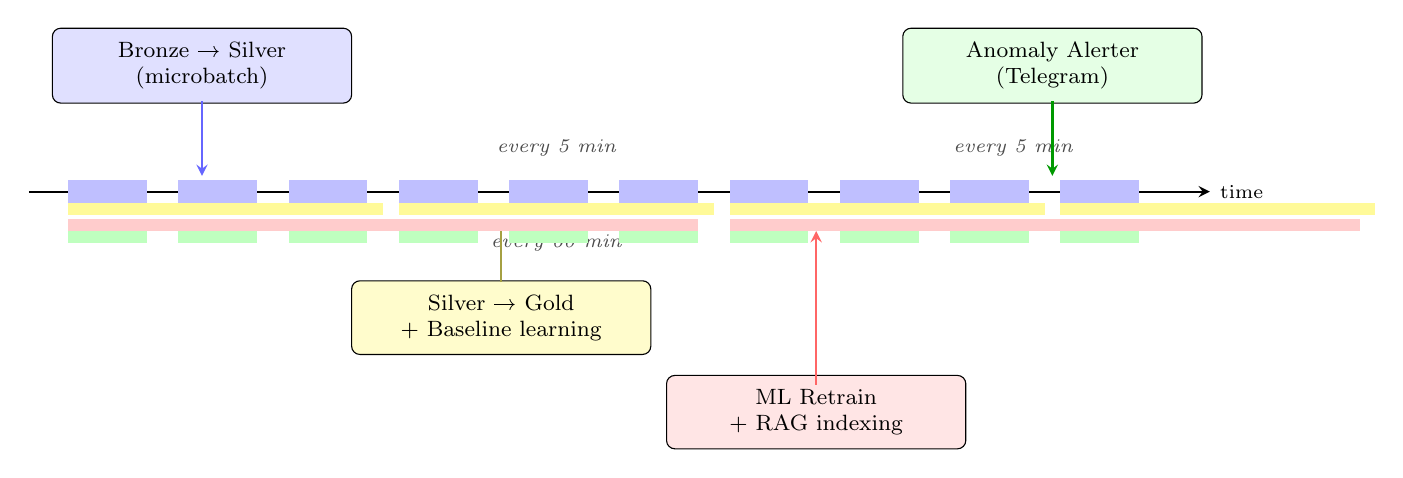
\begin{tikzpicture}[
  >=stealth, font=\small,
  box/.style={draw, rounded corners=3pt, fill=white,
              minimum width=3.8cm, minimum height=0.8cm,
              align=center, font=\footnotesize, inner sep=5pt},
  sched/.style={font=\scriptsize\itshape, gray!60!black},
  arr/.style={->, thick}
]

%% Timeline axis
\draw[thick, ->] (-0.5,0) -- (14.5,0) node[right]{\scriptsize time};

%% Microbatch (every 5 min)
\foreach \x in {0, 1.4, 2.8, 4.2, 5.6, 7.0, 8.4, 9.8, 11.2, 12.6}{
  \fill[blue!25] (\x,-0.15) rectangle (\x+1.0,0.15);
}
\node[sched] at (6.2, 0.55) {every 5 min};
\node[box, fill=blue!12] at (1.7, 1.6) {Bronze → Silver\\(microbatch)};
\draw[arr, blue!60] (1.7,1.15) -- (1.7,0.2);

%% Hourly gold
\foreach \x in {0, 4.2, 8.4, 12.6}{
  \fill[yellow!40] (\x,-0.3) rectangle (\x+4.0,-0.15);
}
\node[sched] at (6.2, -0.65) {every 60 min};
\node[box, fill=yellow!20] at (5.5, -1.6) {Silver → Gold\\+ Baseline learning};
\draw[arr, yellow!60!black] (5.5,-1.15) -- (5.5,-0.35);

%% Retrain (every 6 h)
\foreach \x in {0, 8.4}{
  \fill[red!20] (\x,-0.5) rectangle (\x+8.0,-0.35);
}
\node[sched] at (8.4, -2.45) {every 6 h};
\node[box, fill=red!10] at (9.5, -2.8) {ML Retrain\\+ RAG indexing};
\draw[arr, red!60] (9.5,-2.45) -- (9.5,-0.5);

%% Alerter (every 5 min)
\foreach \x in {0, 1.4, 2.8, 4.2, 5.6, 7.0, 8.4, 9.8, 11.2, 12.6}{
  \fill[green!25] (\x,-0.65) rectangle (\x+1.0,-0.5);
}
\node[sched] at (12.0, 0.55) {every 5 min};
\node[box, fill=green!10] at (12.5, 1.6) {Anomaly Alerter\\(Telegram)};
\draw[arr, green!60!black] (12.5,1.15) -- (12.5,0.2);

\end{tikzpicture}%
}
\caption{Prefect flow schedules: microbatch and alerter run every 5 minutes;
         gold aggregation runs hourly; ML retrain runs every 6 hours.}
\label{fig:batch-flows}
\end{figure}

Figure~\ref{fig:prefect-deployments} shows the Prefect UI confirming all
seven production deployments are active: \texttt{alert\allowbreak-check} and
\texttt{traffic\allowbreak-microbatch} run every 5 minutes,
\texttt{hourly\allowbreak-gold\allowbreak-run} runs hourly,
\texttt{traffic\allowbreak-retrain} and \texttt{rag\allowbreak-index\allowbreak-rebuild}
run every 6 hours, and \texttt{backfill\allowbreak-silver} and
\texttt{bootstrap\allowbreak-infra} run on-demand.

\begin{figure}[htbp]
  \centering
  
\includegraphics[width=\textwidth]{prefect-deployments.png}
  \caption{Prefect 3.x Deployments view: seven active flows covering ingestion,
           batch promotion, model retraining, RAG indexing, and Telegram alerting.}
  \label{fig:prefect-deployments}
\end{figure}

\subsection{Bronze-to-Silver Promotion}

The \texttt{bronze\_to\_silver.microbatch()} function scans the MinIO Bronze
path using a DuckDB glob query
(\texttt{year=*/month=*/day=*/hour=*/*.parquet}), filters for rows not yet
present in the Silver Iceberg table (deduplication by
\texttt{route\_id} + \texttt{timestamp\_utc}), applies type coercion via a
PyArrow schema, and appends to \texttt{silver.traffic\_route}.
The Iceberg table is partitioned by \texttt{day(timestamp\_utc)}, so each
micro-batch write touches only the current day's partition.

\subsection{Silver-to-Gold Aggregation}

The \texttt{silver\_to\_gold.run()} function reads the current hour's Silver
partition and computes per-route hourly aggregates:
\texttt{avg\_duration\_minutes}, \texttt{p95\_duration\_minutes}
(95th percentile using \texttt{numpy.percentile}),
\texttt{avg\_heavy\_ratio}, \texttt{avg\_moderate\_ratio},
and \texttt{max\_severe\_segments}. Results are appended to
\texttt{gold.traffic\_hourly}.

\subsection{Baseline Learning}

The \texttt{baseline\_learning\allowbreak.run()} function queries the entire Gold table
and computes, per \texttt{(route\_id,\allowbreak\ day\_of\_week,\allowbreak\ hour\_of\_day)} triple,
the mean and standard deviation of \texttt{avg\_heavy\_ratio}. An empirical
Z-score threshold is derived from the 99th percentile of the per-route
distribution. These statistics are written to
\texttt{gold.traffic\_baseline} and subsequently loaded by the Online Service
every 6~hours.

\subsection{Anomaly Alerter}

The \texttt{alerter.run()} function queries the PostgreSQL
\texttt{online\_route\_features} table for rows where \texttt{is\_anomaly = TRUE}
and \texttt{updated\_at} is within the last 6 minutes. For each such route,
it calls the Serving API's \texttt{/predict} endpoint to obtain the
IsolationForest score. Only routes where \textbf{both} the Z-score and
IsolationForest signals flag an anomaly (\texttt{both\_anomaly}) trigger a
Telegram notification. A per-route \textbf{30-minute cooldown} prevents
alert flooding during prolonged congestion events.

% ============================================================
\section{ML Service}
\label{sec:impl-ml}
% ============================================================

The \textbf{ML Service} exposes a single FastAPI endpoint \texttt{POST /train}
that trains one \textbf{IsolationForest} model per route and registers each
model in the MLflow Model Registry.

\subsection{Feature Engineering}

Training features are drawn from the Gold table
(\texttt{gold.traffic\_hourly}). The feature vector $\mathbf{x} \in
\mathbb{R}^7$ consists of:

\begin{enumerate}
  \item \texttt{avg\_heavy\_ratio} --- fraction of heavily congested segments.
  \item \texttt{avg\_moderate\_ratio} --- fraction of moderately congested segments.
  \item \texttt{max\_severe\_segments} --- maximum severe segment count in the hour.
  \item $\sin(2\pi \cdot h / 24)$, $\cos(2\pi \cdot h / 24)$ --- cyclical
        encoding of the hour-of-day $h$, so that 23:00 and 00:00 are
        geometrically adjacent~\cite{cyclical_encoding}.
  \item $\sin(2\pi \cdot d / 7)$, $\cos(2\pi \cdot d / 7)$ --- cyclical
        encoding of the day-of-week $d$.
\end{enumerate}

\noindent The cyclical sin/cos transformation is critical: without it, a
linear model would treat Sunday ($d=0$) and Saturday ($d=6$) as maximally
distant, misrepresenting the weekly traffic rhythm.

\subsection{IsolationForest Configuration}

Each per-route model is trained with \texttt{contamination=0.05}
(5\% of training hours assumed anomalous), \texttt{n\_estimators=100}, and
\texttt{random\_state=42}~\cite{liu2008isolation}.
The model is registered in MLflow under the name
\texttt{iforest-\{route\_id\}} with alias \texttt{champion}, enabling
the Serving API to load the latest production-ready model via
\texttt{mlflow.pyfunc.load\_model} with a 1-hour in-process cache
(\texttt{MODEL\_TTL = 3600~s}).

% ============================================================
\section{Serving Layer}
\label{sec:impl-serving}
% ============================================================

The \textbf{Serving Layer} is a \textbf{FastAPI} application that exposes
REST and SSE endpoints consumed by the Next.js frontend.

\subsection{Endpoint Overview}

\begin{table}[htbp]
\centering
\caption{Serving API endpoint summary.}
\label{tab:endpoints}
\begin{tabular}{lll}
\hline
\textbf{Endpoint} & \textbf{Method} & \textbf{Description} \\
\hline
\texttt{/online}                   & GET  & Latest PostgreSQL snapshot per route \\
\texttt{/anomalies}                & GET  & Active anomaly list with history \\
\texttt{/predict}                  & GET  & IsolationForest scores (all routes) \\
\texttt{/anomalies/\{id\}/explain} & GET  & SSE: LLM explanation stream \\
\texttt{/rca}                      & GET  & SSE: root-cause analysis stream \\
\texttt{/chat}                     & POST & SSE: conversational RAG interface \\
\texttt{/events/traffic}           & GET  & SSE: 15-second heartbeat stream \\
\texttt{/metrics}                  & GET  & Heatmaps, zone aggregates \\
\texttt{/telegram/webhook}         & POST & Telegram bot webhook receiver \\
\hline
\end{tabular}
\end{table}

\subsection{SSE Streaming Architecture}

The \texttt{/events/traffic} endpoint loops every 15 seconds, querying
PostgreSQL and the MLflow model cache, then yielding a JSON payload as an SSE
\texttt{data:} frame. This \textit{push} model means the frontend never needs
to poll; a single \texttt{EventSource} connection receives all updates. Token
latency for the LLM explanation endpoints (\texttt{/explain}, \texttt{/rca})
is further minimised by streaming each Ollama token as a separate SSE chunk,
so the user sees the first word within one second regardless of total response
length.

\subsection{RAG-Enriched Inference}

The \texttt{/anomalies/\{route\_id\}/explain} endpoint constructs a
three-part context before calling Ollama:

\begin{enumerate}
  \item \textbf{Static geographic knowledge} (built at startup by
        \texttt{geo\_knowledge.py}): named arterial roads, zone descriptions,
        and HCMC landmark references injected into the system prompt.
  \item \textbf{Live weather} (Open-Meteo API, 15-minute cache): temperature,
        precipitation, wind speed, and WMO weather code for HCMC.
  \item \textbf{RAG context} (ChromaDB): top-$k$ chunks retrieved from two
        collections --- \texttt{anomaly\_events} (indexed hourly by the
        batch pipeline) and \texttt{traffic\_patterns} (indexed every 6
        hours). Retrieval uses \textbf{nomic-embed-text}~\cite{nomic_embed}
        embeddings with cosine similarity.
\end{enumerate}

\noindent The assembled prompt is then streamed to the
\textbf{Qwen2.5:3b}~\cite{qwen25_report} model via the Ollama HTTP API.
This RAG approach~\cite{lewis2020rag} avoids the need to fine-tune the
base model: the LLM reasons over injected facts rather than memorising
traffic patterns, ensuring that explanations remain accurate even as
city traffic evolves week to week.

Figure~\ref{fig:ai-explanation} shows a production anomaly explanation for
\texttt{zone6\_southern\_coastal $\to$ zone5\_western\_periurban} rendered in
Vietnamese. The Qwen2.5:3b model references specific road conditions and
contextualises the anomaly with weather data retrieved from the Open-Meteo
API, demonstrating the RAG pipeline's ability to produce operator-ready,
language-specific explanations.

\begin{figure}[htbp]
  \centering
  
\includegraphics[width=0.85\textwidth]{ai-explanation.png}
  \caption{Production AI Explanation modal for the Coastal $\to$ Western route
           anomaly (Vietnamese output): Qwen2.5:3b generates a contextualised
           explanation referencing weather conditions and route history via RAG.}
  \label{fig:ai-explanation}
\end{figure}

Figure~\ref{fig:ai-chat} shows the conversational \texttt{/chat} SSE
endpoint in action. The user asks about current traffic conditions in
Vietnamese and receives a structured response listing congestion levels for
multiple routes (e.g., Southern Port $\to$ Western 10.9\%, Southern Port
$\to$ Eastern 7.9\%), all generated by the Qwen2.5:3b model over
ChromaDB-retrieved context.

\begin{figure}[htbp]
  \centering
  
\includegraphics[width=0.85\textwidth]{ai-chat.png}
  \caption{Urban Pulse AI Chat interface (Vietnamese): conversational RAG
           endpoint reporting live congestion percentages per route, powered
           by Qwen2.5:3b and the ChromaDB \texttt{traffic\_patterns} collection.}
  \label{fig:ai-chat}
\end{figure}

Figure~\ref{fig:ai-chat-en} demonstrates the same chat endpoint in English.
The model surfaces live weather context alongside congestion data --- here
reporting partly cloudy conditions at 26.8\textdegree C alongside the
Southern Port $\to$ Western Periurban route at 10.9\% heavy ratio ---
confirming that the RAG pipeline correctly retrieves and synthesises both
the Open-Meteo weather feed and the PostgreSQL feature store in a single
response regardless of query language.

\begin{figure}[htbp]
  \centering
  
\includegraphics[width=0.72\textwidth]{ai-chat-english.png}
  \caption{Urban Pulse AI Chat (English): Qwen2.5:3b integrates live weather
           data (26.8\textdegree C, partly cloudy) with congestion metrics
           in a single natural-language response, demonstrating bilingual RAG capability.}
  \label{fig:ai-chat-en}
\end{figure}

\subsection{Dual-Signal Fusion in Serving}

The \texttt{prediction\_service.py} module loads all per-route IsolationForest
models and scores the \textit{current} feature vector reconstructed from
PostgreSQL. The fusion rule is:

\begin{equation}
  \texttt{both\_anomaly} = \texttt{zscore\_anomaly} \;\wedge\; \texttt{iforest\_anomaly}
\end{equation}

Only \texttt{both\_anomaly} routes are escalated to Telegram. This conjunction
rule deliberately trades recall for precision: a route must independently
exceed the statistical threshold \textit{and} be scored as an outlier by the
trained model before an alert is sent.

\subsection{Frontend Dashboard}

The Next.js 15 frontend consumes the SSE stream and renders two primary views.
Figure~\ref{fig:heatmap-zscore} and Figure~\ref{fig:heatmap-both} show the
\textbf{Traffic Metrics heatmap}: a route $\times$ hour grid where each cell
is coloured by congestion severity. Hovering a cell reveals the route
coordinates, Z-score value, and the detector that flagged it
(\texttt{ZSCORE} for a Z-score-only event, \texttt{BOTH} for a dual-signal
confirmation). Figure~\ref{fig:heatmap-zscore} shows the Coastal $\to$
Urban Core route at 08:00 with $Z = 4.22$ (Z-score only), while
Figure~\ref{fig:heatmap-both} shows the Coastal $\to$ Western route at
15:00 with $Z = 2.02$ confirmed by both detectors.

\begin{figure}[htbp]
  \centering
  
\includegraphics[width=\textwidth]{dashboard-heatmap-zscore.png}
  \caption{Traffic Metrics heatmap: tooltip showing a Z-score-only anomaly
           on the Coastal $\to$ Urban Core route at 08:00 ($Z = 4.22$),
           Apr 12--15, 2026.}
  \label{fig:heatmap-zscore}
\end{figure}

\begin{figure}[htbp]
  \centering
  
\includegraphics[width=\textwidth]{dashboard-heatmap-both.png}
  \caption{Traffic Metrics heatmap: tooltip showing a dual-signal anomaly
           (\texttt{BOTH}) on the Coastal $\to$ Western route at 15:00
           ($Z = 2.02$), Apr 12--15, 2026.}
  \label{fig:heatmap-both}
\end{figure}
